\chapter{Constructing Synchronizing Transformations
   \pgsize{20 p.}
}
\label{chap:synchronization}

\todo{Vermeidbarkeit hängt insb. auch von der verwendeten Sprache ab. Z.B. sind Mappings / QVT-R analysierbar, aber Reactions / QVT-O nicht.}

\todo{Ergebnis sollte sein: Synchronisierungseigenschaft ist erreichbar per Konstruktuion}

\mnote{Transformation correctness can be achieved by adhering to the definition}
Transformations are the central artifacts of which a transformation network is composed.
We have introduced them as \emph{synchronizing transformations} in \autoref{def:synchronizingtransformation}, which are combinations of a consistency relation together with a consistency preservation rules that preserves it.
Correctness of such a transformation could then be defined as the property of the consistency preservation rule to preserve consistency of given models according to the consistency relation (cf.\ \autoref{def:synchronizingtransformationcorrectness}).
In theory, a correct transformation can simply be achieved by adhering to that definition.

\mnote{Transformation languages base on unidirectional consistency preservation rules}
Using existing transformation languages, the defined transformations will, however, not follow the definition of a synchronizing transformation.
Transformation languages usually allow the specification of unidirectional consistency preservation rules, i.e., rules that restore consistency by updating one model if the other was modified.
Even if transformation languages allow bidirectional specifications, they still derive unidirectional consistency preservation rules from such a specification, such as forward and backward transformation (which may be incremental or not) derived from \glspl{TGG} rules~\cite{leblebici2014IncrementalTGGSurvey-GTVMT}.
In the following, we refer to such transformations as \emph{ordinary transformations} and give a more precise definition of them later on.
Synchronizing transformation, as we assume in transformation networks, are able to process changes made in both models and, in turn, also produce changes for both models.
This is necessary, because in transformation networks both models involved in a transformation may have been modified due to different sequences of transformations having modified both of them.

\mnote{We want to find requirements to ordinary transformations to be used as synchronizing ones}
In this chapter, we aim to close this gap between synchronizing transformations as required in transformation networks and ordinary transformations with unidirectional consistency preservation rules used by transformation languages.
We investigate which requirements such an ordinary transformation has to fulfill to emulate a synchronizing transformation and thus be used in a transformation network.
This chapter thus constitutes our contribution \contributionref{contrib:correctness:synchronization}, which consists of three subordinate contributions: a discussion of the formal basis for the gap between synchronizing and ordinary transformations, a case distinction for synchronization scenarios in ordinary transformations, and finally techniques to build synchronizing transformations by ordinary ones.
\todo{Finally update goals}
It answers the following research question:

\researchquestionrepeat{rq:correctness:synchronization}

\mnote{Making ordinary transformations synchronizing enables reuse of languages and knowledge}
The benefit of enabling the definition of ordinary transformations that can be used a synchronizing ones instead of providing an approach or language for the specification of synchronizing transformations is that existing and well-researched transformation languages and knowledge about them can be reused.
Additionally, it reduces the complexity, because the definition of two unidirectional consistency preservation rules is less cumbersome than the definition of a single synchronizing transformation, which has to consider all possible combinations of changes in two models.
We will see that this is founded by the insight that only few combinations of changes are problematic and have to be explicitly considered.



%%%
%%% FORMAL GAP IDENTIFICATION
%%%
\section{Gap between Synchronizing and Ordinary Transformations}

We have already introduced that there is both a formal and practical gap between synchronizing transformations, as we have defined as a component of transformation networks, and ordinary transformations, which are unidirectional and non-synchronizing, as used by most transformation languages.
In the following, we first give an example for faulty behavior if we simply used ordinary transformations in a transformation network.
Afterwards, we discuss options to sequentialize ordinary transformations and finally come up with a precise description of the formal gap and a practical approach to close it.

%%
%% MOTIVATING FAULT EXAMPLE WITH ORDINARY TRANSFORMATIONS
%%
\subsection{Behavior of Ordinary Transformations in Networks}
We have already sketched the example of creating a class in UML and Java after adding a component to a \gls{PCM} model in \autoref{chap:introduction:challenges:correctness:synchronization}.
In that scenario, it was possible that for a created \gls{PCM} component first a UML class is generated, which is then transformed into a Java class.
Additionally, the transformation between \gls{PCM} and Java creates another Java class, as it does not consider that there may be another transformation that already created that class.
Such scenarios can lead to the duplication of elements, or, in case of Java, an overwrite of an already created element, because the source file of the class will be placed at the same location in the file system.
Overwriting the previously created file may also overwrite and thus remove information that was already added to that class by the transformations across UML.

\begin{figure}
    \centering
    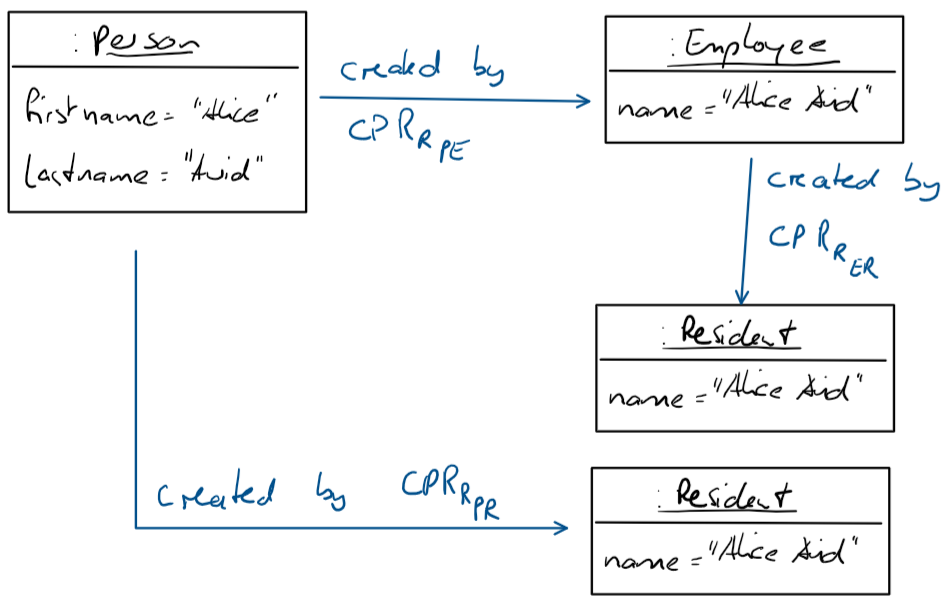
\includegraphics[width=0.8\textwidth]{figures/correctness/synchronization/duplicate_creation_example.png}    
    \caption{Duplicate creation of a resident by two sequences of consistency preservation rules}
    \label{fig:synchronization:duplicate_creation_example}
\end{figure}

An analogous example can be given for the running example of persons, employees and residents depicted in \autoref{fig:networks:three_persons_example}.
We consider the consistency relations $\consistencyrelation{R}{PE}, \consistencyrelation{R}{ER}$ and $\consistencyrelation{R}{PR}$.
As discussed in \autoref{chap:compatibility}, these relations are compatible, thus for any given person, employee or resident, there is a consistent set of models containing it.
Thus, the relations do not prevent transformations from finding consistent models whenever a person, employee or resident is added.
If we now consider ordinary transformations with unidirectional consistency preservation rules, they react to the changes in one model and update another accordingly.
In case of adding a person, this may look as depicted in \autoref{fig:synchronization:duplicate_creation_example}.
For each of the given consistency relations, we assume unidirectional consistency preservation rules that preserve consistency according to them.
They especially create an employee for each added person, and a resident for each created employee and person, respectively.
Since the transformations assume the models to be consistent before applying the changes, they always add a corresponding element when one of the elements is added.
This leads to the situation that both $\consistencypreservationrule{CPR}{\consistencyrelation{CR}{ER},\rightarrow}$ as well as $\consistencypreservationrule{CPR}{\consistencyrelation{CR}{PR},\rightarrow}$ create a resident upon creation of a person.
In consequence, there exist two residents with the same name, which does not fulfill the consistency relations.

It is our goal to find out how such a situation can be avoided by proper definition of consistency preservation rules in existing transformation languages.
A simple solution in this example would have been to look for the existence of elements to create first.
This can either be done by using a trace model, which most existing transformation language use to store corresponding elements, or by searching for an appropriate element in the other model.
Using a trace model, however, has some drawbacks and pitfalls, which we will investigate later.


% \begin{copiedFrom}{DocSym}

% % \section{Binary Transformation Interoperability}

% % Multi-model consistency preservation can be a achieved by combining binary transformations to graphs, %of transformations, 
% % with the transformations being executed transitively.
% % Since all binary transformations are developed independently of each other, it is necessary that they interoperate properly in a \emph{non-intrusive} way, thus without the necessity for the developer to understand and modify them, which we refer to as \emph{black-box combination}.

% Even under the assumption that, in contrast to our introductory motivation, all specifications are free of contradictions, it is easy to see that problems arise when combining binary transformations by transitively executing them.
% For example, consider the relations in \autoref{fig:prologue:binary_combination_example}.
% If a component is added to the \ac{ADL}, causing a \ac{UML} class creation due to \ref{fig:prologue:binary_combination_example:R1}, which in turn causes a Java class creation due to \ref{fig:prologue:binary_combination_example:R2}, the transformation for relation \ref{fig:prologue:binary_combination_example:R3} does not know that an appropriate class was already created, if the transformations are treated as black boxes.
% Consequently, the transformation will create the same class again, which may override the existing one, depending on the implementation and execution order.
% A simple solution for this example would be to have all transformations use a common trace model and check for existing elements before creating them in a transformation.
% Nevertheless, independently developed transformations will usually not assume that %this only applies if the transformation considers possibly preexisting transformation results, which it will not do in general if it does not assume other transformations to create corresponding elements.
% other transformations may already have created corresponding elements.
% Additionally, the trace model must allow the transformation engine to retrieve transitive traces.
% However, it is unclear if transitive resolution of traces can always be performed, as it can depend on whether the transitive trace belongs the considered consistency relation or another.
% %If, in another scenario, the transformation in the example was actually supposed to create an additional class, it would have to ignore the existing trace.

% As can be seen in the example, especially the correct handling of trace information in interdependent transformations has to be researched.
% This applies not only to element creations, but also other change types, such as attribute or reference changes, especially if they are multi-valued.
% In our thesis, we will therefore apply transitively executed binary transformations in different case studies to identify these and potential further problems.
% We then want to come up with a catalog of such problems %preventing the black-box combination of transformations 
% together with solution patterns for them.
% For example, to avoid duplicate element creations, a simple pattern could be to always check for already existing traces for that consistency relation in the transformations.
% In consequence, the integration of those patterns into a transformation language or the application of them as a transformation developer is supposed to achieve black-box combinability of the transformations.

% \end{copiedFrom} % DocSym


\subsection{Options for Transformation Sequentialization}

\mnote{Existing synchronization supports arbitrary conflicting concurrent changes}
Some existing work already proposed strategies to synchronize concurrent changes between two models.
For example, some work proposes techniques for processing concurrent changes with \glspl{TGG}~\cite{hermann2012concurrentSynchronization-FASE,orejas2020IncrementalConcurrentSynchronization-FASE}, whereas others define specific algorithms for a general notion of synchronizing transformations according to our given definition~\cite{xiong2013SynchronizingConcurrentUpdates-SoSym,xiong2009parallelUpdates-ICMT}.
All these approaches, however, deal with the more general case that any changes may have been made to the models.
That especially includes conflicting updates by one or more user, which need to be resolved.
Such a resolution may lead to the necessity of reverting one of the changes.

\mnote{Transformation networks only produce specific concurrency situations}
We are, however, in the special situation that transformations do not perform arbitrary changes and that changes of other transformations may need to be revised, but not reverted.
For example, it may be necessary to update an attribute value again, because the interval of consistent values of the currently executed transformation is smaller than the one of a transformation executed before.
It will, however, not be necessary to completely revert the modification of the attribute value, because the modification was necessary for another transformation to restore consistency, thus the causal change for which consistency was restored, needs to be reverted as well.
Finally, this would result in reverting a user change, which should never happen.

\mnote{We assume compatibility of transformations}
In fact, we assume transformations to be compatible according to \autoref{def:compatibility}, which excludes contradictions in their consistency relations that may prevent transformations from being able to find a consistent result for specific changes.
This assumptions reduces the potential conflicts that may occur when changes of different transformations need to be synchronized.

\todo{Go on here}



A consistency preservation rule according to \autoref{def:consistencypreservationrule} receives two models and two changes, one for each of the models, and returns two changes, i.e.:
\begin{align*}
    \consistencypreservationrule{\consistencyrelation{CR}{}} : (\metamodelinstanceset{M}{1}, \metamodelinstanceset{M}{2}, \changeuniverse{\metamodel{M}{1}}, \changeuniverse{\metamodel{M}{2}}) \rightarrow (\changeuniverse{\metamodel{M}{1}}, \changeuniverse{\metamodel{M}{2}})
\end{align*}
\todo{Maybe add this to correctness formalization: Give example why we need that: both models can be modified due to network, both may need to be modified because if in both models something is added that needs to be reflected in the other, both have to be changed to restore consistency, without reverting one of the changes.}
We used this rather general notion of a consistency preservation rule between two metamodels to support that both models may have been modified, which is inevitable in a transformation network.
Additionally, both models may need to be modified to properly consistency.
It would, however, be a cumbersome task to define the behavior of the transformation, or more precisely its consistency preservation rule, for all potential pairs of changes in both models.
Furthermore, existing transformation languages usually specify unidirectional consistency preservation rules, thus they only support the propagation of changes made in one model to the other, but not to process changes made to both models at once.
\begin{align*}
    \consistencypreservationrule{\consistencyrelation{CR}{},\rightarrow} : (\metamodelinstanceset{M}{1}, \metamodelinstanceset{M}{2}, \changeuniverse{\metamodel{M}{1}}) \rightarrow \changeuniverse{\metamodel{M}{2}}\\
    \consistencypreservationrule{\consistencyrelation{CR}{},\leftarrow} : (\metamodelinstanceset{M}{1}, \metamodelinstanceset{M}{2}, \changeuniverse{\metamodel{M}{2}}) \rightarrow \changeuniverse{\metamodel{M}{1}}
\end{align*}

\mnote{First option: Independent execution and merge}
In consequence, we usually have two unidirectional consistency preservation rules that define how changes are propagated from one model to the other and vice versa, but this is not equivalent to a synchronizing transformation.
Imagine models $\model{m}{1}$ and $\model{m}{2}$ and changes to them $\change{\metamodel{M}{1}}$ and $\change{\metamodel{M}{2}}$.
If we now applied two unidirectional consistency preservation rules individually, we would apply the first to $\model{m}{1},\model{m}{2}$ and $\change{\metamodel{M}{1}}$, returning $\change{\metamodel{M}{2}}'$, and the second one to $\model{m}{1},\model{m}{2}$ and $\change{\metamodel{M}{2}}$, returning $\change{\metamodel{M}{1}}'$.
It is, however, not guaranteed whether $\tupled{\change{\metamodel{M}{1}}' \concatfunction \change{\metamodel{M}{1}}(\model{m}{1}), \change{\metamodel{M}{2}}' \concatfunction \change{\metamodel{M}{2}}(\model{m}{2})}$ is consistent.

\mnote{Second option: Sequential execution}
Another option would be to sequentialize the execution, thus first generating $\change{\metamodel{M}{2}}'$ as before by applying one consistency preservation rule to $\model{m}{1},\model{m}{2}$ and $\change{\metamodel{M}{1}}$.
Afterwards, the second rule is applied to $\change{\metamodel{M}{1}}(\model{m}{1}),\change{\metamodel{M}{2}}'(\model{m}{2})$ and $\change{\metamodel{M}{2}}$.
This means that $\change{\metamodel{M}{2}}$ is not applied to $\model{m}{2}$ anymore, to which the changes were made originally, but needs to applied to $\change{\metamodel{M}{2}}'(\model{m}{2})$.
It is, however, not clear whether the change can still be applied to that state, i.e., whether $\change{\metamodel{M}{2}}$ is defined for $\change{\metamodel{M}{2}}'(\model{m}{2})$.
An example may be that $\change{\metamodel{M}{2}}'$ removes an element from $\model{m}{2}$, which $\change{\metamodel{M}{2}}$ changes.
\todo{Revise change definition to be partial}

We, however, want to ensure that both original changes are applied to the models and consistency preservation rules can react to them.



\subsection{The Formal Gap of Synchronizing and Ordinary Transformations}

\begin{itemize}
    \item We assume consistency preservation rules according to fine-grained consistency relations introduced for compatibility
    \item So a synchronizing transformation considers fine-grained relations, in fact a transformation then consists of multiple relations, two for each fine-grained relation (each direction). Their combination induces the \modellevelconsistencyrelation for the two metamodels.
    \item Although the consistency preservation rule may in practice also be defined in terms fine-grained rules, which together with the fine-grained consistency rules then forms what is often called \emph{transformation rules}, we do not need to have a more fine-grained notion here.
    \item The transformation then is still correct as defined before, when the preservation rule preserves consistency to the relation, but now according to all fine-grained relations (and thus also the induced monolithic one) instead to the single model-level one.
    \item To reflect the notion of unidirectional consistency preservation rules, as often defined in transformation languages, which are still synchronizing, i.e., are able to react to changes made to both models, we may define:
\end{itemize}
\begin{align*}
    \consistencypreservationrule{\consistencyrelationset{CR}_{\rightarrow},\rightarrow} : (\metamodelinstanceset{M}{1}, \metamodelinstanceset{M}{2}, \changeuniverse{\metamodel{M}{1}}, \changeuniverse{\metamodel{M}{2}}) \rightarrow \changeuniverse{\metamodel{M}{2}})\\
    \consistencypreservationrule{\consistencyrelationset{CR}_{\leftarrow},\leftarrow} : (\metamodelinstanceset{M}{1}, \metamodelinstanceset{M}{2}, \changeuniverse{\metamodel{M}{1}}, \changeuniverse{\metamodel{M}{2}}) \rightarrow \changeuniverse{\metamodel{M}{1}})
\end{align*}

Now we can define correctness as before as the rule for one direction ensuring that models are consistent to that direction.
We may also define the following property:
\begin{definition}{Inverse-preserving Synchronizing Transformation}%Unidirectional Consistency Preservation Rule}
    Let T be a synchronizing transformation for two metamodels $\metamodel{M}{1}$ and $\metamodel{M}{2}$, consisting of the two consistency rule sets $\consistencyrelationset{CR}_{\rightarrow}$ and $\consistencyrelationset{CR}_{\leftarrow}$ and consistency preservation rules $\consistencypreservationrule{\consistencyrelationset{CR}_{\rightarrow},\rightarrow}$ as well as $\consistencypreservationrule{\consistencyrelationset{CR}_{\leftarrow},\leftarrow}$.
    T is \emph{inverse-preserving} if, and only if, executing one of the consistency preservation rules ensures that all consistency relations of the opposite direction, to which the models were consistent before, the resulting models are still consistent to.
    For one of the directions, this is given by the following (the other direction analogously):
    \begin{align*}
        & \forall \model{m}{1} \in \metamodelinstanceset{M}{1} : \forall \model{m}{2} \in \metamodelinstanceset{M}{2}: \forall \change{\metamodel{M}{1}} \in \changeuniverse{\metamodel{M}{1}} : \forall \change{\metamodel{M}{2}} \in \changeuniverse{\metamodel{M}{2}} : \\
        & 
        \forall \consistencyrelation{CR}{} \in \consistencyrelationset{CR}_{\leftarrow}:
        \tupled{\change{\metamodel{M}{2}}(\model{m}{2}),\change{\metamodel{M}{1}}(\model{m}{1})} \consistenttomath \consistencyrelation{CR}{} \\
        & 
        \Rightarrow \tupled{\consistencypreservationrule{\consistencyrelationset{CR}_{\rightarrow},\rightarrow}(\model{m}{1},\model{m}{2},\change{\metamodel{M}{1}},\change{\metamodel{M}{2}})(\model{m}{2}), \change{\metamodel{M}{1}}(\model{m}{1})} \consistenttomath \consistencyrelation{CR}{}
    \end{align*}
\end{definition}

This is a reasonable property, because the consistency relations in both directions are usually not disaligned, but only give the freedom to define different behaviors in both directions, such as more options in one direction than in the other to support different kinds of abstraction.
However, it should not be the case that preserving consistency in one direction violates consistency relations in the other direction if transformations are defined properly.

The given definition ensures that if a transformation is inverse-preserving, then executing the two unidirectional transformations one after another restore consistency to all consistency relations, because no directional rule is allowed to violate consistency that was already ensured in the other direction.
\todo{Define, how execution "one after another" looks like}

\begin{proposition}
    \todo{show that a inverse-preserving synchronizing transformation results in consistent state after both directions are executed once}
\end{proposition}

In fact, it is not easy to ensure that two unidirectional transformations are inverse-preserving, even if the consistency relations in both directions are the same, which we will also see in our evaluation of errors in \autoref{chap:errors}.
This problem, however, already arises when defining bidirectional transformations.
They may derive two unidirectional preservation rules from one specifications, thus that they are inherently inverse-preserving, or they may allow individual specification of the directions and provide some support for checking that they conform to each other, e.g., in the sense that they are inverse-preserving.
This is, however, an isolated and existing topic of research and a challenge that already has to be solved for a single bidirectional transformation rather than a network, which is why we do not discuss this problem in more detail here.

Still, there is a gap to practical approaches for defining transformations, as existing approaches do not support the synchronization scenario, i.e., they are not able to process changes in both models, but only in one of them.
Actually, existing transformations usually assume that changes are either made by the developer and are then to be propagated to the other model by the transformation, or they are made by the transformation in reaction to changes to the other model.
The case that user modify multiple models is sometimes also referred to as a synchronization scenario (although the term is sometimes even used for the simple case of incremental update).
If we consider that scenario, we will refer to it as \emph{concurrent editing} to avoid confusion.
Although the two cases have in common that both instead of only one model involved in a transformation may have been modified, they have a specific difference.
While user changes to both models can be arbitrary conflicting, changes performed by other transformations in a network should, in the best case, not be conflicting, especially if the underlying relations are compatible, as discussed in \autoref{chap:compatibility}.
For example, if a user changes an element A, whose information needs to be propagated to element B, but removes element B as well, this cannot be easily resolved, apart from potentially removing element A as well.
However, as we know from existing approaches for concurrent editing with tools like Git, conflict resolution is not an easy task~\todo{add cite for difficulty of conflict resolution}.
Such a scenario may not occur in a transformation network, because if transformations remove elements that are to be updated by others, there will obviously be some conflicts in the transformations, potentially imposed by contradictions in the underlying consistency relations.

An ordinary unidirectional consistency preservation rule looks as follows:
\begin{align*}
    \consistencypreservationrule{\consistencyrelationset{CR}_{\rightarrow},\rightarrow} : (\metamodelinstanceset{M}{1}, \metamodelinstanceset{M}{2}, \changeuniverse{\metamodel{M}{1}}) \rightarrow \changeuniverse{\metamodel{M}{2}}
\end{align*}
Thus, the rule is not synchronizing, i.e., it does not consider that the second model was modified as well.

If we pass the changed second model, i.e., given models $\model{m}{1},\model{m}{2}$ and changes $\change{\metamodel{M}{1}},\change{\metamodel{M}{2}}$, we call $\consistencypreservationrule{\consistencyrelationset{CR}_{\rightarrow},\rightarrow}(\model{m}{1},\change{\metamodel{M}{2}}(\model{m}{2}),\change{\metamodel{M}{1}})$.
Then, in general, the behavior of the function is undefined, as in \autoref{def:consistencypreservationrulecorrectness}, we only required the function to return a change such that applying all changes produces consistent models if the original models were consistent.
In this case, however, the given models are not consistent to each other.


\subsection{Closing the Gap}

We thus want to achieve a slight adaptation of those unidirectional consistency preservation rules, such that they support the case that the second model has already been modified.
Informally speaking, we want to emulate unidirectional synchronizing rules with non-synchronizing ones.
Additionally, we want to ensure that such a rule that is inverse-preserving for consistent inputs is also inverse-preserving for the case that the second model was already modified, such that executing both rules consecutively ensures consistency to the relations in both directions, like we have shown for a pair of inverse-preserving unidirectional synchronizing consistency preservation rules.
So the question is:
What has to be considered if a consistency preservation rule $\consistencypreservationrule{\consistencyrelationset{CR}_{\rightarrow},\rightarrow}$ shall be able to process the input $\tupled{\model{m}{1},\change{\metamodel{M}{2}}\model{m}{2},\change{\metamodel{M}{1}}}$, return $\change{\metamodel{M}{2}}'$, such that $\tupled{\model{m}{1},\model{m}{2}}$ is consistent to $\consistencyrelationset{CR}_{\rightarrow}$, as well as $\tupled{\change{\metamodel{M}{1}}(\model{m}{1}),\change{\metamodel{M}{2}}' \concatfunction \change{\metamodel{M}{2}}(\model{m}{2})}$ is consistent to $\consistencyrelationset{CR}_{\rightarrow}$, and that it is inverse-preserving for that input as well.

To find out what has to be done to achieve that, we consider the possible combinations of changes made to $\model{m}{1}$ and $\model{m}{2}$ that the consistency preservation rule may need to consider.
For each combination of changes, we need to find out whether:
\begin{enumerate}
    \item The result is still consistent to $\consistencyrelationset{CR}_{\rightarrow}$
    \item The process is inverse-preserving, i.e., no relation in $\consistencyrelationset{CR}_{\leftarrow}$ that was fulfilled before is violated afterwards
\end{enumerate}

Since we consider the practical realization of such preservation rules with ordinary transformation languages, we also specifically consider the changes that can be processed by those transformation languages.
Thus, we focus on the types of changes that can be performed in EMOF-based and conforming Ecore-based models.

\todo{Go on here: map this to synchronizing ones and the inverse-preserving property}



\begin{itemize}
    \item Define unidirectional consistency preservation rules as above
    \item Define correctness of unidirectional consistency preservation rules
    \item Say that we want to investigate what happens when we apply CPR to m1, d(m2) with m1, m2 consistent instead of to m1, m2
\end{itemize}



Even if we consider that one may only define a consistency preservation rule, which then induces the consistency relation as its image, thus being correct by construction, the rule may not behave as expected.


Problem statement: Problem is a practical one, not a theoretical one.
Ordinary transformations may be correct if used on their own (according to Stevens), but in context of a transformation network, when other transformation have modified the "target" model as well, they do not lead to a consistent result anymore, i.e., they are not correct.
Start with example of duplicated creation and overwrite.

Define ordinary transformations to take deltas in model 1 and produce deltas in model 2
Say that unidirectional synchronizing transformations take deltas in both models and update the deltas in one of them.
Refer to fine-grained formalization regarding compatibility, where consistency relations are directional, thus each directional preservation rule preserves consistency according to the consistency relations in one direction.
Having synchronizing unidirectional transformation, executing both preserves consistency to both unidirectional consistency relations. However, their must be some kind of conformance of the unidirectional transformation to each other (define how this conformance looks like!), so that executing each once does not lead to violations in the other direction. In general, that may not be possible. In fact, each unidirectional transformation should consider the unidirectional consistency relations of both directions.

So:
Ordinary unidirectional transformation for Rr: m1, m2, d1 -> d2, such that (d1(m1), d2(m2)) consistent to all relations in Rr (Rl respectively)
Synchronizing unidirectional transformation: m1, m2, d1, d2 -> d2', such that (d1(m1), d2'(m2)) consistent to all relations Rr and consistent to all relations in Rl to which is was consistent before (thus no violation of further consistency relations)

Direct consequence: Executing one transformation after the other ensures that models are consistent to alle relations in Rr and relation

Based on that, we derive how we can use languages that take deltas in model 1 and produce them in model 2 to emulate synchronizing unidirectional transformations that are able to manage deltas in both models and produce deltas in one of them.
For that, we make the case distinction and derive the creation pattern.
For each change merge case, we consider that we somehow "merge" the changes. In general, the change of the transformation to m2 will overwrite the previous change to m2. Then we consider that there is another consistency relation affected by the new change. We show whether/why not the other consistency relation can be violated by that change and discuss how to avoid that.




%%%
%%% CASE DISTINCTION 
%%%
\section{Synchronization Scenarios in Ordinary Transformations}





%%%
%%% AVOIDANCE PATTERNS
%%%
\section{Synchronization of Ordinary Transformation}
Goal: Avoidance strategies for interoperability mistakes, i.e. achieving synchronization of transformations (MA Torsten / Timur)
\label{chap:prevention:interoperability}

\begin{copiedFrom}{ICMT}

% FORMERLY: \subsection{Matching Elements in Operationalizations}
\subsection{Matching Elements}
\label{chap:prevention:interoperability:matching}

To avoid failures due to mistakes at the operationalization level, transformations must respect that other transformations may have already created elements.
In the binary case, this is unnecessary.
A single incremental \ac{BX} can assume that elements are either created by the user, %and then are input of the transformations
or were created by the transformation itself.
To identify corresponding elements, transformation languages usually use trace models, which are created by the transformations.
When \acp{BX} are combined to networks, %elements may also be created by other transformations.
%In consequence, 
direct trace links may be missing because a sequence of other transformations created the elements and trace links only indirectly across elements in other models.
%Thus, it is necessary to establish direct trace links between corresponding elements.´
In this scenario, corresponding elements can be matched by information at three levels:
%Such element matching can be performed on three levels:
\begin{enumerate}
    \item \emph{Explicit unique}: The information that elements correspond is unique and represented explicitly, e.g., within a trace model. %Existing transformation languages usually use this technique.
    \item \emph{Implicit unique}: The information that elements correspond is unique, but represented implicitly, e.g., in terms of key information within the models such as element names. %types and element names.
    \item \emph{Non-unique}: If no unique information exists, heuristics must be used, e.g. based on ambiguous information or transitive resolution of indirect trace links.
\end{enumerate}
\todo{Give examples for each case to show that they actually occur}

Indirect trace links, which link elements transitively across other models, usually exist for elements that correspond, because other transformations have already created them.
Nevertheless, indirect trace links cannot be used to unambiguously identify such elements.
An element can correspond to multiple elements in another model, which is why most transformation languages offer tagging of trace links with additional information to identify the correct element.
%For example, a component in an architecture description could be mapped to two classes in an object-oriented design, one providing the component implementation and one providing utilities.
%The relevant corresponding element can be retrieved if the traces are tagged with the information that one class is the implementation and one is a utility.
For example, a language may tag trace links with the transformation rule they were instantiated in.
This is helpful in the bidirectional case, but when links are resolved transitively, these tags have been created by other, independently developed transformations, and are thus unknown.
%If such tags would be considered, transformations would depend on tags of other transformations and could thus not be developed independently anymore.
Therefore, resolving indirect trace links is only a heuristic, but does not unambiguously retrieve corresponding elements.

% Explain how to match rules on three different levels, what the levels can provide etc.

% \begin{enumerate}
%     \item Direct Correspondences
%     \item Key information
%     \item Heuristics: Indirect correspondences, potentially ambiguous information
% \end{enumerate}

Finally, it is up to the transformation engine or the transformation developer %, depending on the provided abstraction level, 
to ensure that elements are correctly matched.
In contrast to the bidirectional case, direct trace links cannot be assumed in case of networks of \acp{BX}.
Therefore, key information within the models must always be considered to identify matching elements.
Whenever direct trace links or unique key information exists, relevant elements can be unambiguously matched.
In all other cases, heuristics must be used, which potentially leads to failures.

\end{copiedFrom} % ICMT



%%% 
%%% SUMMARY
%%%
\section{Summary}

\begin{insight}[Synchronization]
    When constructing synchronizing transformations, both models may have been and need to be modified in contrast to ordinary bidirectional transformations, which update only one of the models.
    Having ordinary transformations and consistency preservation rules for both directions, executing only one or one after another does not necessarily lead to a consistent result, thus the transformations are not correct in context of a transformation network when both models may have been modified.
    We, however, found that their sequential execution leads to a consistent result for all possible combinations of changes, if identity of elements is handled correctly.
    In contrast to ordinary incremental transformation, which assume that elements were created by the user or the transformation itself, in a transformation network other transformation may have already created appropriate elements.
    In consequence, a transformation needs to identify if an element already exists upon its creation.
    To achieve that, it needs to define key information for identifying that element.
    With that addition, executing ordinary incremental transformations in both directions, each of the consistency preservation rules being correct, the emulated synchronizing transformation is correct.
    In consequence, synchronizing transformations can be constructed with existing transformation languages not considering synchronization and without knowing about other transformations to combine them with.
\end{insight}

\todo{Is this true? We can have cycles there, so it may not be correct. Just consider the confluence case?}